% data processing
\section{Data processing}
This section describes data processing of the microseismic continuous time series of seismic data in order to perform the FAST algorithm described in the paper by Yoon et al, 2015 \cite{yoon2015earthquake}. 
%\newline

First, Yoon et al., 2015 downsample their continuous time series data from 100 samples/second to 20 samples/second. This makes the Nyquist frequency of their time series 10 Hz. We downsample our continuous time series as well, but not to the same Nyquist frequency as the paper. Our time series is the result of microseismic activity, and it has higher frequency content than the macroseismic data used by Yoon et al. We downsample from 1000 samples/second to 500 samples/second. This leaves us with a Nyquist frequency of 250 Hz. 
%\newline

Next, Yoon et al. create a spectrogram from the continuous time series data. They begin by dividing the time series data into windows of 200 samples each, with a lag of 2 samples, which means an overlap between the windows of 198 samples. In other words, the windows are 10 seconds long, with a lag of 0.1 seconds. Our time series is considerably shorter than theirs, 20 seconds long compared to 3600 seconds long, so we divided our time series into windows of 50 samples each, with a lag of 2 samples, which means an overlap between windows of 48 samples. This means we created windows that are 0.025 seconds long, with a lag of 0.001 second. 
%\newline

Yoon et al. apply a Hamming tapering window to each time series window. They do not specify the length of this tapering window. We apply a symmetric Hamming tapering window that is equal to the length of each time series window, which is 50 samples. The MATLAB function hamming was used to do this.
%\newline

Yoon et al. take the short time Fourier transform (STFT) of the time series by computing the Fourier transform of each tapered window. The paper does not specify how many sampling points are used to calculate this discrete Fourier transform. We use 127 points. These Fourier transforms are then combined to create the STFT for the entire continuous time series.
%\newline
Finally, Yoon et al. generate the spectrogram by calculating the power of the STFT. In other words, they calculate the squared amplitude of the complex-valued STFT. We do the same thing with our STFT.
%\newline

Next, Yoon et al. downsample the spectrogram so that it has only 32 frequency bins. We do the same thing to our spectrogram. In order to do a successful wavelet transform later, the number of frequency bins needs to be a power of 2. The spectrogram computed from the continuous time series data is shown in Figure \ref{fig:spec}.
% \newline

Yoon et al. separate the spectrogram into what they call "spectral images" by dividing it into overlapping windows in the time domain. They used 100 samples per spectral image, with a lag of 10 samples, which means an overlap of 90 samples. In other words, they had windows 10 seconds long, with a lag of 1 second. We used windows of 128 samples, with a lag of 5 samples, which means an overlap of 123 samples. We end up with windows that are 0.512 s long, with a lag of 0.02 s. This gives a total of 969 spectral images.
% \newline

Yoon et al. downsample each spectral image in the time domain to 64 samples. We also downsample to 64 samples in the time domain, leaving spectral images with dimensions 32 samples by 64 samples. Each of these dimensions must be a power of 2 for the wavelet transform, which is performed next, to work. 
A sample spectral image is shown in Figure \ref{fig:specim}. 
\begin{figure*}
	\centering
%\epsfysize=50mm 
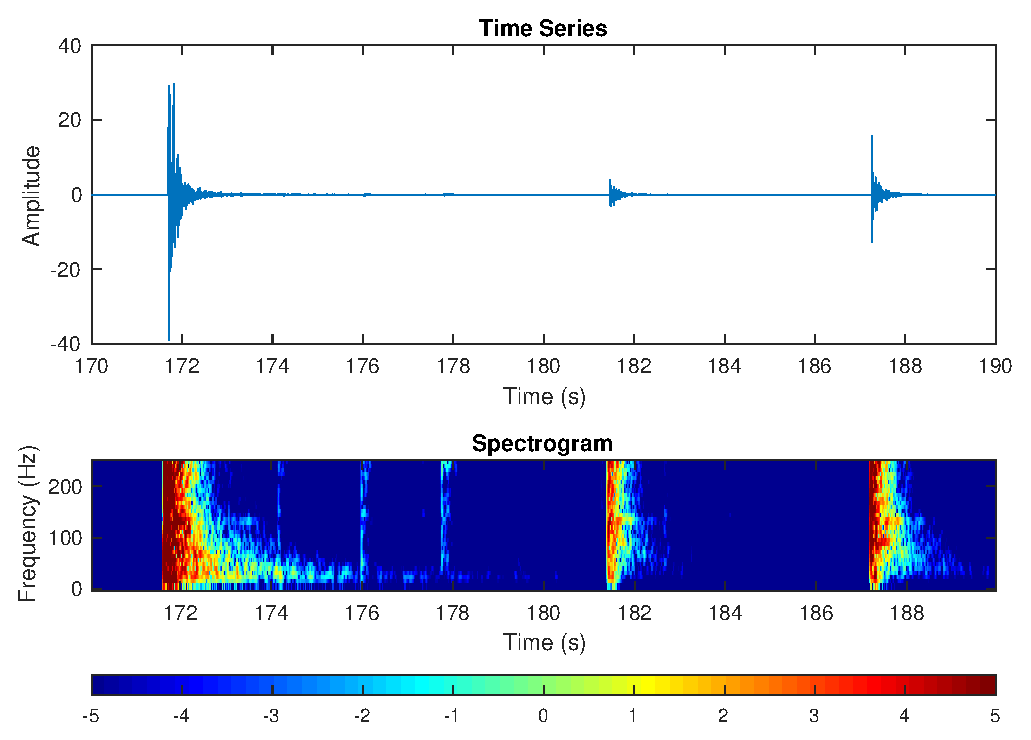
\includegraphics[width=0.7\textwidth]{sampleSpectrogram}
\caption{(Upper figure) Original continuous time series data. (Lower figure) Spectrogram created using the STFT of the continuous time series data. Amplitude is plotted on a log scale. The vertical component was used here.}
\label{fig:spec}
\end{figure*}

\begin{figure}
	\centering
%\epsfysize=50mm 
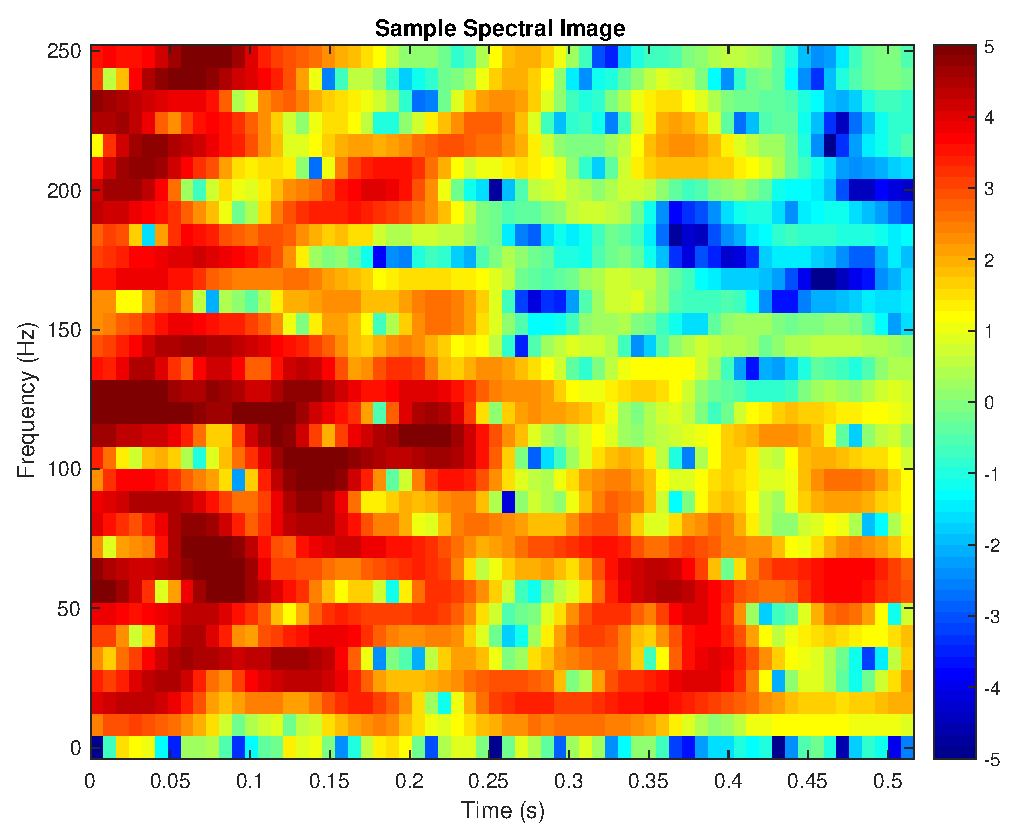
\includegraphics[width=0.5\textwidth]{sampleSpectralImage}
\caption{Sample spectral image taken from the spectrogram.}
\label{fig:specim}
\end{figure}
